\setstretch{1.5}
\subsection{Παράδειγμα ταξινόμησης \en{mergesort}}
\mbox{}
Η ταξινόμηση \emph{\en{mergesort}} είναι ένας αλγόριθμος που κατατάσσεται στην κατηγορία \en{Divide and Conquer}. Πρόκειται για έναν αναδρομικό αλγόριθμο στο οποίο
δοθέντος ενός διανύσματος προς ταξινόμηση, αυτό διαιρείται σε δύο υποσύνολα και για κάθε υποσύνολο εφαρμόζεται η ίδια διαδικασία ταξινόμησης. Όταν ολοκληρωθεί τα δυο υποσύνολα ενώνονται ξανά σε ένα. Η διαδικασία περιγράφεται στο παρακάτω διάγραμμα\cite{wiki_mergesort}

\begin{figure}[h]
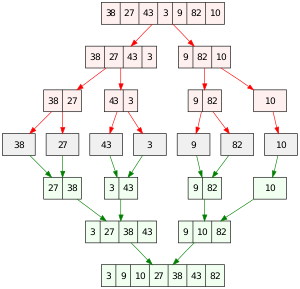
\includegraphics[width=0.4\textwidth]{mergesort}
\centering
\captionsetup{justification=centering, singlelinecheck=false}
	\caption{\en{Mergesort} παράδειγμα}
\label{fig:mergesort}
\end{figure}


\subsubsection{Περιγραφή κοινού τμήματος αλγορίθμου ταξινόμησης \en{mergesort}}
\mbox{}

\selectlanguage{english}
\begin{spacing}{1.0}
\begin{lstlisting}[showstringspaces=false, language=C++, caption={\en{Mergesort: verify()}} , frame=tb]{Name}
 static void verify(int *a, int size)
 {
     for (size_t i = 1; i < size; ++i) {
         if (a[i] < a[i-1]) {
             std::cout << "Verification failed! Aborting ..."
              << std::endl;
             exit(1);
         }
     }

     std::cout << "Successful verification" << std::endl;
 }


\end{lstlisting}
\end{spacing}
\selectlanguage{greek}

\clearpage
\selectlanguage{english}
\begin{spacing}{0.8}
\begin{lstlisting}[language=C++, caption={\en{Mergesort: merge()\cite{merge}}} , frame=tb]{Name}
 void merge(int arr[], int l, int m, int r)
 {
     int i, j, k;
     int n1 = m - l + 1;
     int n2 = r - m;

     /* create temp arrays */
     int *L = new int[n1];
     int *R = new int[n2];

     /* Copy data to temp arrays L[] and R[] */
     for (i = 0; i < n1; i++)
         L[i] = arr[l + i];
     for (j = 0; j < n2; j++)
         R[j] = arr[m + 1 + j];

     /* Merge the temp arrays back into arr[l..r]*/
     i = 0; // Initial index of first subarray
     j = 0; // Initial index of second subarray
     k = l; // Initial index of merged subarray
     while (i < n1 && j < n2) {
         if (L[i] <= R[j]) {
             arr[k] = L[i];
             i++;
         }
         else {
             arr[k] = R[j];
             j++;
         }
         k++;
     }

     /* Copy the remaining elements of L[], if there
     are any */
     while (i < n1) {
         arr[k] = L[i];
         i++;
         k++;
     }

     /* Copy the remaining elements of R[], if there
     are any */
     while (j < n2) {
         arr[k] = R[j];
         j++;
         k++;
     }

     delete []L;
     delete []R;
 }


\end{lstlisting}
\end{spacing}
\selectlanguage{greek}


\clearpage
\selectlanguage{english}
\begin{spacing}{1.5}
\begin{lstlisting}[showstringspaces=false, language=C++, caption={\en{Mergesort: main()}} , frame=tb]{Name}
 int main(int argc, char **argv)
 {
     Opts o;
     parseArgs(argc, argv, o);

     int *arr = new int[o.size];
     fill_random_array(arr, o.size);
     //int arr[] = { 12, 11, 13, 5, 6, 7 };

     auto start = omp_get_wtime();
     mergeSort_wrapper(arr, 0, o.size - 1);
     auto end = omp_get_wtime();
     std::cout << "Execution time: " << std::fixed << end-start <<
         std::setprecision(5) << std::endl;
     if (o.verify) {
         verify(arr, o.size);
     }
     return 0;
 }

\end{lstlisting}
\end{spacing}
\selectlanguage{greek}



\clearpage

\subsubsection{Σειριακή εκτέλεση}
\selectlanguage{english}
\begin{spacing}{0.6}
\begin{lstlisting}[language=C++, caption={\en{Mergesort:} \el{Σειριακή Εκτέλεση}}, frame=tb]{Name}
 void mergeSort(int arr[], int l, int r)
 {

     if (l < r) {
         // Same as (l+r)/2, but avoids overflow for
         // large l and h
         int m = l + (r - l) / 2;

         // Sort first and second halves
         mergeSort(arr, l, m);
         mergeSort(arr, m + 1, r);

         merge(arr, l, m, r);
     }
 }

 void mergeSort_wrapper(int *arr, int lhs, int rhs)
 {
     mergeSort(arr, lhs, rhs);
 }
\end{lstlisting}
\end{spacing}
\selectlanguage{greek}

\begin{table}[h]
    \centering
    \caption{\en{Mergesort}: Επιλογές μεταγλώττισης \en{Alt1, Alt2}}
    \label{my-label}
    \begin{tabular}{
    |p{0.1\textwidth}
    | >{\centering\arraybackslash}p{0.8\textwidth}
    |}
    \hline
 {\textbf{\en{Label}}} & \textbf{\en{Options}} \\ \hline
     \textbf{\en{Alt1}} & \en{-fopt-info-vec=builds/alt1.log -O2 -fno-inline -fno-tree-vectorize -fopenmp -o ./builds/Alt1} \\ \hline
      \textbf{\en{Alt2}} & \en{-fopt-info-vec=builds/alt2.log -O2 -fno-inline -ftree-vectorize -fopenmp -o ./builds/Alt2} \\ \hline
    \end{tabular}
\end{table}

\begin{table}[h]
    \centering
    \caption{\en{Mergesort}: Αποτελέσματα \en{Alt1, Alt2}}
    \label{my-label}
    \resizebox{0.6\textwidth}{!} {
    \begin{tabular}{|p{0.20\textwidth}
    | >{\centering\arraybackslash}p{0.12\textwidth}
    | >{\centering\arraybackslash}p{0.12\textwidth}
    |}
    \hline
    \multirow{2}{*}{\textbf{\shortstack{Μέγεθος\\προβλήματος}}} & \multicolumn{2}{|c|}{\textbf{Χρόνοι εκτέλεσης \en{(sec)}}} \\ \cline{2-3} 
               & \textbf{\en{Alt1}} & \textbf{\en{Alt2}}\\ \hline
     2000000 & 0.557 & 0.505 \\ \cline{1-3} 
     3000000 & 0.838 & 0.775 \\ \cline{1-3} 
     4000000 & 1.145 & 1.098 \\ \cline{1-3} 
     5000000 & 1.392 & 1.315 \\ \cline{1-3} 
     6000000 & 1.714 & 1.587 \\ \cline{1-3} 
     7000000 & 1.999 & 1.882 \\ \cline{1-3} 


    \end{tabular}}
\end{table}
\clearpage


\subsubsection{Παραλλαγή με \en{task}}
Στο παράδειγμα της παραγράφου, οι ρουτίνες \en{mergesort} εισάγονται σε εργασίες με σκοπό τη παράλληλη εκτέλεσή τους. Παρόλο που η επίλυση εξάγει σωστά αποτελέσματα, εμφανίζει μεγάλη καθυστέρηση στο χρόνο εκτέλεσης, όπως φαίνεται στον πίνακα που ακολουθεί, γιαυτό δεν αυξάνεται το μέγεθος του προβλήματος.
\selectlanguage{english}
\begin{spacing}{0.4}
\begin{lstlisting}[language=C++, caption={\en{Mergesort: task - taskwait}} , frame=tb]{Name}
 void mergeSort(int arr[], int l, int r)
 {
     if (l < r) {
         // Same as (l+r)/2, but avoids overflow for
         // large l and h
         int m = l + (r - l) / 2;

         // Sort first and second halves
 #pragma omp task
         {
             mergeSort(arr, l, m);
         }

 #pragma omp task
         {
             mergeSort(arr, m + 1, r);
         }
 #pragma omp taskwait
         merge(arr, l, m, r);
     }
 }

 void mergeSort_wrapper(int *arr, int lhs, int rhs)
 {
 #pragma omp parallel
 #pragma omp single
     {
         mergeSort(arr, lhs, rhs);
     }
 }

\end{lstlisting}
\end{spacing}
\selectlanguage{greek}

\begin{table}[h]
    \centering
    \caption{\en{Mergesort}: Επιλογές μεταγλώττισης \en{Alt3, Alt4}}
    \label{my-label}
	\resizebox{0.9\textwidth}{!} {
    \begin{tabular}{
    |p{0.1\textwidth}
    | >{\centering\arraybackslash}p{0.8\textwidth}
    |}
    \hline
 {\textbf{\en{Label}}} & \textbf{\en{Options}} \\ \hline
     \textbf{\en{Alt3}} & \en{-fopt-info-vec=builds/alt3.log -O2 -fno-inline -fno-tree-vectorize -fopenmp -o ./builds/Alt3} \\ \hline
      \textbf{\en{Alt4}} & \en{-fopt-info-vec=builds/alt4.log -O2 -fno-inline -ftree-vectorize -fopenmp -o ./builds/Alt4} \\ \hline
    \end{tabular}}
\end{table}

\begin{table}[h]
    \centering
    \caption{\en{Mergesort}: Αποτελέσματα \en{Alt3, Alt4}}
    \label{my-label}
    \resizebox{0.6\textwidth}{!} {
    \begin{tabular}{|p{0.20\textwidth}
    | >{\centering\arraybackslash}p{0.12\textwidth}
    | >{\centering\arraybackslash}p{0.12\textwidth}
    |}
    \hline
    \multirow{2}{*}{\textbf{\shortstack{Μέγεθος\\προβλήματος}}} & \multicolumn{2}{|c|}{\textbf{Χρόνοι εκτέλεσης \en{(sec)}}} \\ \cline{2-3} 
               & \textbf{\en{Alt3}} & \textbf{\en{Alt4}}\\ \hline
     2000000 & 28.648 & 27.689 \\ \cline{1-3} 
    \end{tabular}}
\end{table}

\clearpage


\subsubsection{Παραλλαγή με \en{task} (2)}
\mbox{}
\selectlanguage{english}
\begin{spacing}{0.7}
\begin{lstlisting}[language=C++, caption={\en{Mergesort: task - depend}}, frame=tb]{Name}
 void mergeSort(int arr[], int l, int r)
 {
     int x, y;
     if (l < r) {
         // Same as (l+r)/2, but avoids overflow for
         // large l and h
         int m = l + (r - l) / 2;

         // Sort first and second halves
 #pragma omp task depend(in: x)
         {
             mergeSort(arr, l, m);
         }

 #pragma omp task depend(in: y)
         {
             mergeSort(arr, m + 1, r);
         }
 #pragma omp task depend(out: x, y)
         {
             merge(arr, l, m, r);
         }
 #pragma omp taskwait
     }
 }

 void mergeSort_wrapper(int *arr, int lhs, int rhs)
 {
 #pragma omp parallel
 #pragma omp single
     {
         mergeSort(arr, lhs, rhs);
     }
 }
\end{lstlisting}
\end{spacing}
\selectlanguage{greek}

\begin{table}[h]
    \centering
    \caption{\en{Mergesort}: Επιλογές μεταγλώττισης \en{Alt5, Alt6}}
    	\resizebox{0.8\textwidth}{!} {
    \label{my-label}
    \begin{tabular}{
    |p{0.1\textwidth}
    | >{\centering\arraybackslash}p{0.8\textwidth}
    |}
    \hline
 {\textbf{\en{Label}}} & \textbf{\en{Options}} \\ \hline
     \textbf{\en{Alt5}} & \en{-fopt-info-vec=builds/alt5.log -O2 -fno-inline -fno-tree-vectorize -fopenmp -o ./builds/Alt5} \\ \hline
      \textbf{\en{Alt6}} & \en{-fopt-info-vec=builds/alt6.log -O2 -fno-inline -ftree-vectorize -fopenmp -o ./builds/Alt6} \\ \hline
    \end{tabular}}
\end{table}

\begin{table}[h]
    \centering
    \caption{\en{Mergesort}: Αποτελέσματα \en{Alt5, Alt6}}
    \label{my-label}
    \resizebox{0.6\textwidth}{!} {
    \begin{tabular}{|p{0.20\textwidth}
    | >{\centering\arraybackslash}p{0.12\textwidth}
    | >{\centering\arraybackslash}p{0.12\textwidth}
    |}
    \hline
    \multirow{2}{*}{\textbf{\shortstack{Μέγεθος\\προβλήματος}}} & \multicolumn{2}{|c|}{\textbf{Χρόνοι εκτέλεσης \en{(sec)}}} \\ \cline{2-3} 
               & \textbf{\en{Alt5}} & \textbf{\en{Alt6}}\\ \hline
     2000000 & 36.707 & 42.075 \\ \cline{1-3} 
    \end{tabular}}
\end{table}

\clearpage

\subsubsection{Παραλλαγή με \en{task} (3)}
Σε μια ακόμα προσπάθεια επίλυσης με \en{tasks}, εισάγεται η φράση \emph{\en{final}} με σκοπό τη μείωση του παραγόμενου αριθμού εργασιών. Λόγω του μεγάλου μεγέθους διανύσματος οι εργασίες που δημιουργούνται είναι τόσες, που το κόστος της δημιουργίας τους επιβαρύνει σημαντικά στο συνολικό χρόνο εκτέλεσης του προβλήματος.
\selectlanguage{english}
\begin{spacing}{0.8}
\begin{lstlisting}[language=C++, caption={\en{Mergesort: task - taskwait - critical}} , frame=tb]{Name}
int LIMIT = omp_get_num_threads();
int num_rec = 0;

/* l is for left index and r is right index of the
sub-array of arr to be sorted */
void mergeSort(int arr[], int l, int r)
{
#pragma omp critical
    {
        ++num_rec;
    }

    int x, y;
    if (l < r) {
        // Same as (l+r)/2, but avoids overflow for
        // large l and h
        int m = l + (r - l) / 2;
        // Sort first and second halves
#pragma omp task final(num_rec > LIMIT)
        {
            mergeSort(arr, l, m);
        }

#pragma omp task final(num_rec > LIMIT)
        {
            mergeSort(arr, m + 1, r);
        }
#pragma omp taskwait
        {
            merge(arr, l, m, r);
        }
    }
}

void mergeSort_wrapper(int *arr, int lhs, int rhs)
{
#pragma omp parallel
#pragma omp single
    {
        mergeSort(arr, lhs, rhs);
    }
}
\end{lstlisting}
\end{spacing}
\selectlanguage{greek}
\clearpage
\begin{table}[h]
    \centering
    \caption{\en{Mergesort}: Επιλογές μεταγλώττισης \en{Alt9, Alt10}}
    \label{my-label}
    \begin{tabular}{
    |p{0.1\textwidth}
    | >{\centering\arraybackslash}p{0.8\textwidth}
    |}
    \hline
 {\textbf{\en{Label}}} & \textbf{\en{Options}} \\ \hline
     \textbf{\en{Alt9}} & \en{-fopt-info-vec=builds/alt9.log -O2 -fno-inline -fno-tree-vectorize -fopenmp -o ./builds/Alt9} \\ \hline
      \textbf{\en{Alt10}} & \en{-fopt-info-vec=builds/alt10.log -O2 -fno-inline -ftree-vectorize -fopenmp -o ./builds/Alt10} \\ \hline
    \end{tabular}
\end{table}

\begin{table}[h]
    \centering
    \caption{\en{Mergesort}: Αποτελέσματα \en{Alt9, Alt10}}
    \label{my-label}
    \resizebox{0.7\textwidth}{!} {
    \begin{tabular}{|p{0.20\textwidth}
    | >{\centering\arraybackslash}p{0.12\textwidth}
    | >{\centering\arraybackslash}p{0.12\textwidth}
    |}
    \hline
    \multirow{2}{*}{\textbf{\shortstack{Μέγεθος\\προβλήματος}}} & \multicolumn{2}{|c|}{\textbf{Χρόνοι εκτέλεσης \en{(sec)}}} \\ \cline{2-3} 
               & \textbf{\en{Alt9}} & \textbf{\en{Alt10}}\\ \hline
     2000000 & 2.612 & 1.759 \\ \cline{1-3}
     3000000 & 3.929 & 2.460 \\ \cline{1-3} 
     4000000 & 5.395 & 5.331 \\ \cline{1-3} 
     5000000 & 6.683 & 3.893 \\ \cline{1-3} 
     6000000 & 7.916 & 7.394 \\ \cline{1-3} 
 
    \end{tabular}}
\end{table}

\clearpage

\subsubsection{Παραλλαγή με \en{task} (4)}
Η τελευταία παραλλαγή της λύσης του προβλήματος, προκύπτει μετά από αρκετές προσπάθειες αποτυχημένων εκτελέσεων. Η δημιουργία νέων εργασιών παύει όταν το μέγεθος του διαιρεμένου διανύσματος είναι μικρότερο από μια προκαθορισμένη τιμή. Σε περίπτωση που το μέγεθος είναι μικρότερο από \en{WORKLOAD} τότε η εργασία ενσωματώνεται στη προηγούμενη.
\selectlanguage{english}
\begin{spacing}{0.8}
\begin{lstlisting}[language=C++, caption={\en{Mergesort: taskgroup - taskyield}} , frame=tb]{Name}
 #define WORKLOAD 16000

 /* l is for left index and r is right index of the
 sub-array of arr to be sorted */
 void mergeSort(int arr[], int l, int r)
 {

     if (l < r) {
         // Same as (l+r)/2, but avoids overflow for
         // large l and h
         int m = l + (r - l) / 2;
 #pragma omp taskgroup
         {
 #pragma omp task shared(arr) untied if (r - l >= WORKLOAD)
             mergeSort(arr, l, m);
 #pragma omp task shared(arr) untied if (r - l >= WORKLOAD)
             mergeSort(arr, m+1, r);
 #pragma omp taskyield
         }
         merge(arr, l, m, r);
     }
 }

 void mergeSort_wrapper(int *arr, int lhs, int rhs)
 {
 #pragma omp parallel
 #pragma omp single
     mergeSort(arr, lhs, rhs);
 }


\end{lstlisting}
\end{spacing}
\selectlanguage{greek}
\begin{table}[h]
    \centering
    \caption{\en{Mergesort}: Επιλογές μεταγλώττισης \en{Alt11, Alt12}}
    \label{my-label}
    \begin{tabular}{
    |p{0.1\textwidth}
    | >{\centering\arraybackslash}p{0.8\textwidth}
    |}
    \hline
 {\textbf{\en{Label}}} & \textbf{\en{Options}} \\ \hline
     \textbf{\en{Alt11}} & \en{-fopt-info-vec=builds/alt11.log -O2 -fno-inline -fno-tree-vectorize -fopenmp -o ./builds/Alt11} \\ \hline
      \textbf{\en{Alt12}} & \en{-fopt-info-vec=builds/alt12.log -O2 -fno-inline -ftree-vectorize -fopenmp -o ./builds/Alt12} \\ \hline
    \end{tabular}
\end{table}
\clearpage

\begin{table}[h]
    \centering
    \caption{\en{Mergesort}: Αποτελέσματα \en{Alt11, Alt12}}
    \label{my-label}
    \resizebox{0.7\textwidth}{!} {
    \begin{tabular}{|p{0.20\textwidth}
    | >{\centering\arraybackslash}p{0.12\textwidth}
    | >{\centering\arraybackslash}p{0.12\textwidth}
    |}
    \hline
    \multirow{2}{*}{\textbf{\shortstack{Μέγεθος\\προβλήματος}}} & \multicolumn{2}{|c|}{\textbf{Χρόνοι εκτέλεσης \en{(sec)}}} \\ \cline{2-3} 
               & \textbf{\en{Alt11}} & \textbf{\en{Alt12}}\\ \hline
     2000000 & 0.178 & 0.146 \\ \cline{1-3}
     3000000 & 0.209 & 0.194 \\ \cline{1-3} 
     4000000 & 0.288 & 0.247 \\ \cline{1-3} 
     5000000 & 0.357 & 0.324 \\ \cline{1-3} 
     6000000 & 0.395 & 0.374 \\ \cline{1-3} 
     7000000 & 0.489 & 0.467 \\ \cline{1-3} 
 
    \end{tabular}}
\end{table}

\paragraph{Παρατηρήσεις}
\ \\
Η παράγραφος αυτή περιέχει τη μοναδική υλοποίηση με χρήση \en{OpenMP} που οι χρόνοι εκτέλεσης είναι μικρότεροι από αυτούς της σειριακής. Η χρήση \emph{\en{OpenMP}} όπως φάνηκε από τις προηγούμενες προσπάθειες μπορεί να προκαλέσει μείωση των επιδόσεων καθώς το κόστος δημιουργίας νέων εργασιών μπορεί να είναι μεγαλύτερο από το χρόνο εκτέλεσής τους.


\begin{figure}[h]
\begin{tabular}{*{2}{>{\centering\arraybackslash}b{\dimexpr0.5\linewidth-2\tabcolsep\relax}}}
\resizebox{0.5\textwidth}{!} {
\begin{tikzpicture}[state/.append style={minimum size=7mm}]
     \begin{axis}[
         xlabel={Μέγεθος διανυσμάτων},
         ylabel={Χρόνος εκτέλεσης},
         xmin=2e6, xmax=7e6,
         ymin=0, ymax=2,
         xtick={ 2e6, 3e6, 4e6, 5e6, 6e6, 7e6},
         ytick={ 0, 0.5, 1, 1.5, 2},
         legend pos=north west,
        % ymajorgrids=true,
        % grid style=dashed,
     ] 
 	
 	\addplot[ color=blue, mark=triangle,]
      coordinates {
          (2e6, 0.557)(3e6, 0.838)
          (4e6, 1.145)(5e6, 1.392)(6e6, 1.714)
          (7e6, 1.999)
 	};
 	\addlegendentry{\en{Alt1}}
 	
 	\addplot[ color=red, mark=square,]
      coordinates {
          (2e6, 0.178)(3e6, 0.209)(4e6, 0.288)
          (5e6, 0.357)(6e6, 0.395)(7e6, 0.489)
 	};
 	\addlegendentry{\en{Alt11}}
 	
     \end{axis}
 \end{tikzpicture}}

 \caption{\en{MergeSort:} Σύγκριση \en{Alt1, Alt11}}
    &
\renewcommand{\arraystretch}{1.1}
\resizebox{0.5\textwidth}{!} {
\begin{tabular}{c|c}
Μέγεθος & Ποσοστό μείωσης χρόνου (\%)  \\
\hline
\en{2000000} & 68 \\
\en{3000000} & 75 \\
\en{4000000} & 74 \\
\en{5000000} & 74 \\
\en{6000000} & 77 \\
\en{7000000} & 75 \\


\end{tabular}}
\captionof{table}{\en{Mergesort:} Ποσοστιαία σύγκριση \en{Alt1} και \en{Alt11}}
\end{tabular}
\end{figure}
